\documentclass{article}
\usepackage{fullpage}
\usepackage{multicol}
\usepackage{graphicx}

\begin{document}
\begin{center}
{\bf 930590352}
	
CSCI 243 Spring 2011 HW0
\end{center}
\begin{enumerate}
\item With only two variables, we can construct the following truth table:	
	\begin{center}
	\begin{tabular}{ | c | c | c | c | c |}
		\hline
	  	$p$ & $q$ & $p \land q$ & $p \oplus q$ & $\neg p \rightarrow q $\\  \hline
		$T$ & $T$ & $T$ & $F$ & $T$ \\
		$T$ & $F$ & $F$ & $T$ & $T$ \\
		$F$ & $T$ & $F$ & $T$ & $T$ \\
		$F$ & $F$ & $F$ & $F$ & $F$ \\ \hline
	\end{tabular}
	\end{center}

\item It's an identity matrix!
	\begin{center}
	\[
	I =
	\left[
	 \begin{array}{c c c c}
		1 & 0 & \cdots & 0 \\
		0 & 1 & \cdots & 0 \\
		\vdots & \vdots & \ddots & \vdots \\
		0 & 0 & \cdots & 1
	 \end{array}
	\right]
	\]
	\end{center}

\item Here is my awesome picture from xfig, which was 3 inches by 2 inches, and is centered and scaled to 50\% of the width of my text!
	\begin{center}
		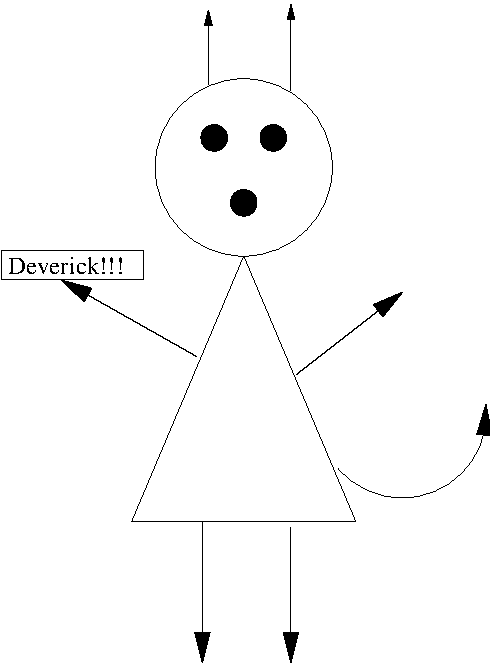
\includegraphics[width=.5 \textwidth] {930590352hw0pic}
	\end{center}
	\begin{center}
		Figure 1: Figures love captions. So do we.
	\end{center}

\item We can use the Binomial Theorem (which we will study later) to expand $(x+y)^4$:
	
	\begin{eqnarray*}
		(x+y)^4 &=& \sum_{j=0}^{4}{4 \choose j}x^{4-j}y^j \\
		&=& {4 \choose 0}x^4 + {4 \choose 1}x^3y + {4 \choose 2}xy^3 + {4 \choose 4}y^4 \\
		&=& x^4 + 4x^3y + 6x^2y^2 + 4xy^3 + y^4
	\end{eqnarray*}

\item If you do not allow repetition, you can select exactly $\frac{n!}{r!(n-r)!}$ combinations of $r$ elements from a set of n elements.

\item Let $s$ represent the number of points you earn in this class.  Then there is a function $L(s)$ that determines your letter grade. Fortunately the follwing is not the definition of $L(s)$ that we will use in this class:
	\[
		L(s) = \left\{
		\begin{array}{l l}
		A+ & \quad :s \geq 97 \\
		A  & \quad :93 \leq s < 97 \\
		A- & \quad :90 \leq s < 93 \\
		F  & \quad :s < 90
		\end{array} \right.
	\]
\item We are going to talk about lots of mathy things in this class, including:
	\begin{enumerate}
		\item counting
		\item induction
		\item functions
	\end{enumerate}

	Of course, some of it will be about other things, such as:
	
	\begin{itemize}
	 \begin{multicols}{2}	
		\item graphs 
		\item trees
		\item formal languages
		\item turing machines
	 \end{multicols}
	\end{itemize}

	Oh wait, those are kinda mathy too. Oh well, we'll have fun!

\end{enumerate}
\end{document}

